\documentclass[border=20pt]{standalone}
\usepackage{tikz}
\usetikzlibrary{matrix,calc,shapes}
\tikzset{
  treenode/.style = {shape=rectangle, rounded corners,
                     draw, anchor=center,
                     text width=30mm, align=center,
                     top color=white, bottom color=blue!20,
                     inner sep=2mm},
  slab/.style   = {treenode, bottom color=green!40},
  slab3/.style   = {slab,text width=60mm},
  slab2/.style   = {slab,text width=45mm},
}
\begin{document}
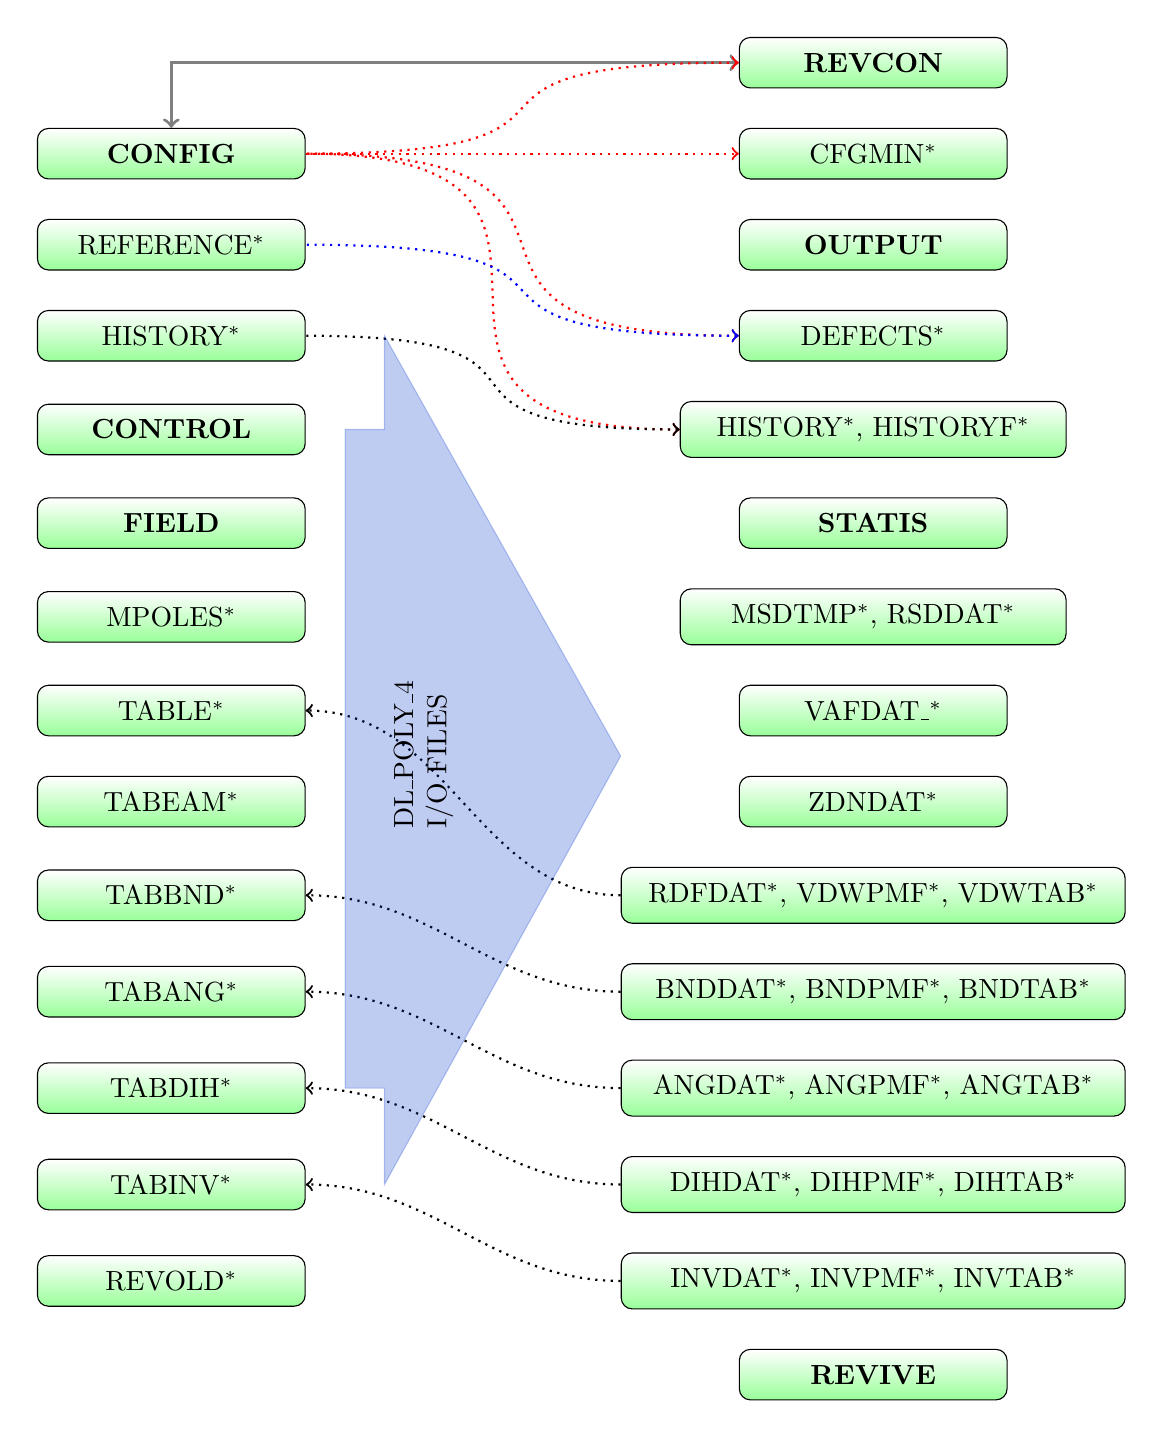
\begin{tikzpicture}[-latex]
  \matrix (chart)
    [
      matrix of nodes,
      column sep      = 40mm,
      row sep         = 5mm,
      column 1/.style = {nodes={slab}},
      column 2/.style = {nodes={slab}}
    ]
    {
                                &  {\bf REVCON}    \\
      {\bf  CONFIG}             &  CFGMIN$^*$       \\
      REFERENCE$^*$                &  {\bf OUTPUT}  \\
      HISTORY$^*$                  & DEFECTS$^*$         \\
      {\bf CONTROL}             & |[slab2]|HISTORY$^*$, HISTORYF$^*$ \\
      {\bf FIELD} &     {\bf STATIS}        \\
      MPOLES$^*$   &    |[slab2]|   MSDTMP$^*$, RSDDAT$^*$         \\
      TABLE$^*$        &  VAFDAT\_$^*$      \\
      TABEAM$^*$       &  ZDNDAT$^*$ \\
      TABBND$^*$       & |[slab3]| RDFDAT$^*$, VDWPMF$^*$, VDWTAB$^*$  \\
      TABANG$^*$       & |[slab3]| BNDDAT$^*$, BNDPMF$^*$, BNDTAB$^*$  \\
      TABDIH$^*$       & |[slab3]| ANGDAT$^*$, ANGPMF$^*$, ANGTAB$^*$  \\
      TABINV$^*$       & |[slab3]| DIHDAT$^*$, DIHPMF$^*$, DIHTAB$^*$  \\
      REVOLD$^*$       & |[slab3]| INVDAT$^*$, INVPMF$^*$, INVTAB$^*$  \\
                       &  {\bf REVIVE}  \\
    };
     \draw[<->,very thick,black!50!white]   (chart-2-1)  |- (chart-1-2);
     \draw[ ->,dotted, thick,red]   (chart-2-1)  -- (chart-2-2);
     \draw[ <-,dotted, thick,red]   (chart-4-2) to [out = 180, in = 0, looseness = 2](chart-2-1);
     \draw[ <-,dotted, thick,red]   (chart-1-2) to [out = 180, in = 0, looseness = 2](chart-2-1);
     \draw[ <-,dotted, thick,red]   (chart-5-2) to [out = 180, in = 0, looseness = 2](chart-2-1);
     \draw[ <-,dotted, thick,blue]   (chart-4-2) to [out = 180, in = 0, looseness = 2](chart-3-1);
     \draw[ <-,dotted, thick,black]   (chart-5-2) to [out = 180, in = 0, looseness = 2](chart-4-1);
     \draw[ ->,dotted, thick,black]   (chart-10-2) to [out = 180, in = 0, looseness = 1](chart-8-1);
     \draw[ ->,dotted, thick,black]   (chart-11-2) to [out = 180, in = 0, looseness = 1](chart-10-1);
     \draw[ ->,dotted, thick,black]   (chart-12-2) to [out = 180, in = 0, looseness = 1](chart-11-1);
     \draw[ ->,dotted, thick,black]   (chart-13-2) to [out = 180, in = 0, looseness = 1](chart-12-1);
     \draw[ ->,dotted, thick,black]   (chart-14-2) to [out = 180, in = 0, looseness = 1](chart-13-1);
     \filldraw[opacity=0.25,green!20!blue]
     ([xshift=5mm]chart-12-1.east)--([xshift=5mm]chart-5-1.east)--
     ([xshift=10mm]chart-5-1.east)--([xshift=10mm]chart-4-1.east)--
     ([xshift=-15mm]$ 0.5*(chart-9-2.west) + 0.5*(chart-8-2.west) $)--
     ([xshift=10mm]chart-13-1.east)--([xshift=10mm]chart-12-1.east)
     --cycle;
     \node [black,opacity=1,rotate=90] at ([xshift=15mm]chart-8-1.east)
     {\begin{minipage}{30mm}
       DL\_POLY\_4\\I/O FILES
     \end{minipage}
     };
   \end{tikzpicture}
\end{document}
